\input format.tex

\usepackage{graphicx}
\graphicspath{{cores/}}
\usepackage{setspace}

\newcolumntype{K}[1]{>{\centering\arraybackslash}p{#1}}

\begin{document}

\vspace*{6mm}

\noindent\fcolorbox{topcolor}{topcolor}{
\parbox[c][1cm]{\textwidth}{
\begin{center}
\fontsize{18pt}{\baselineskip}\selectfont\color{white}{\bf {肠道益生菌检测结果}}
\end{center}
}
}


%% 各章节
\setlength{\arrayrulewidth}{1pt}
\fontsize{8pt}{11pt}\selectfont
\color{black70}

\vspace*{3mm}

\fontsize{11pt}{13pt}\selectfont
\noindent\begin{tabular}{p{4.8cm}p{5.2cm}}
\parbox[c]{\hsize}{\vskip7pt 姓名:Jack \vskip7pt} & 年龄:1 \\
\parbox[c]{\hsize}{\vskip7pt 样本编码:tptest003 \vskip7pt} & 送检机构:湘雅附三体检中心 \\
\end{tabular}

\begin{LRaside2}{\bf 您本次肠道益生菌总评分如下}
\begin{center}
\setlength{\unitlength}{1cm}
\begin{picture}(20,2.6)(0,-0.8)
\put(10.4073684210526,0.55){
\includegraphics[scale=1]{straw_l4.pdf}}
\put(0.5,-0.2){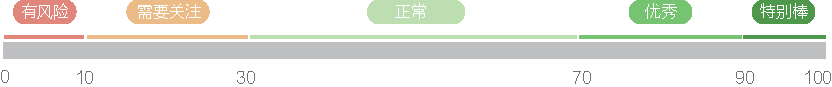
\includegraphics[scale=1]{baohulibar03.pdf}}
\end{picture}
\indent\fontsize{9pt}{11pt}\selectfont\bf {综合您本次肠道益生菌检测,您本次益生菌检测总评分为
{\fontsize{13pt}{14pt}\selectfont\color{level4} 72分},优秀
}

\includegraphics[scale=1]{underline.pdf}
\end{center}
{\par\fontsize{9pt}{11pt}\selectfont\bf {肠道保护力优秀,请您继续保持。肠道益生菌评分越高,说明您的肠道越健康;反之,肠
道益生菌评分越低,则说明您的肠道微生态环境越值得关注。}}
\end{LRaside2}

\vspace*{-2mm}
\hspace*{12.5cm}
\raisebox{-0.4ex}{
\includegraphics{drop_l4.pdf}}
\fontsize{9pt}{11pt}\selectfont {本次检测结果}

\vspace*{5mm}

\noindent\fontsize{11pt}{12pt}\selectfont {\bf 综合健康建议}
\noindent
\fontsize{8pt}{11pt}\selectfont
\setlength{\arrayrulewidth}{.5pt}
\begin{center}
\begin{tabular}{K{1.3cm}K{13.6cm}}
\hline

\parbox[c][2.5cm]{.95\hsize}{
\noindent

\includegraphics[scale=1.0]{diet.pdf}
}
 &
%\hspace*{1mm}
\parbox{\hsize}{
\vspace*{0.5mm}
\begin{spacing}{1.5}
{
\includegraphics[scale=1.0]{xiaoyuandian.pdf}\fontsize{8.5pt}{10pt}\selectfont \ 饮食以奶为主,可根据月龄和宝宝发育情况酌情添加辅食,辅食的添加建议由少到多、由稀到稠,逐步增加辅食的种类,如米粉、蛋羹、胡萝卜汁等。辅食加工宜清淡无盐、软烂易消化。 \\}
{
\includegraphics[scale=1.0]{xiaoyuandian.pdf}\fontsize{8.5pt}{10pt}\selectfont \ 控制食用糖、含糖饮料等高糖食物。}
\end{spacing}
} \\
\hline

\parbox[c][2.5cm]{.95\hsize}{
\noindent

\includegraphics[scale=1.0]{probiotics.pdf}
}
 &
%\hspace*{1mm}
\parbox{\hsize}{
\vspace*{0.5mm}
\begin{spacing}{1.5}
{
\includegraphics[scale=1.0]{xiaoyuandian.pdf}\fontsize{8.5pt}{10pt}\selectfont \ 您平时可适量多喝酸奶。酸奶营养丰富易吸收,含有大量活性益生菌的酸奶(如保加利亚乳杆菌、BB-12),能帮助调节肠道酸碱值,抑制有害菌的生长,增强人体免疫力。}
\end{spacing}
} \\
\hline

\parbox[c][2.5cm]{.95\hsize}{
\noindent

\includegraphics[scale=1.0]{prebiotics.pdf}
}
 &
%\hspace*{1mm}
\parbox{\hsize}{
\vspace*{0.5mm}
\begin{spacing}{1.5}
{
\includegraphics[scale=1.0]{xiaoyuandian.pdf}\fontsize{8.5pt}{10pt}\selectfont \ 您可选择性补充益生元,如0.8g {/} 100mL的低聚半乳糖、0.2g {/} 100mL的低聚果糖、儿童合生元等,能帮助益生菌在肠道内增殖,增加有益物质的产生,有利于增强肠道屏障功能,促进肠道健康。 \\}
{
\includegraphics[scale=1.0]{xiaoyuandian.pdf}\fontsize{8.5pt}{10pt}\selectfont \ 不适合摄入膳食纤维制剂。}
\end{spacing}
} \\
\hline

\end{tabular}
\end{center}


\end{document}

